\documentclass[letterpaper,11pt]{article}
\oddsidemargin -1.0cm \textwidth 17.5cm

\usepackage[utf8]{inputenc}
\usepackage[activeacute,spanish, es-lcroman]{babel}
\decimalpoint
\usepackage{amsfonts,setspace}
\usepackage{amsmath}
\usepackage{amssymb, amsmath, amsthm}
\usepackage{comment}
\usepackage{float}
\usepackage{amssymb}
\usepackage{dsfont}
\usepackage{anysize}
\usepackage{multicol}
\usepackage{enumerate}
\usepackage{graphicx}
\usepackage[left=1.5cm,top=2cm,right=1.5cm, bottom=1.7cm]{geometry}
\setlength\headheight{1.5em} 
\usepackage{fancyhdr}
\usepackage{multicol}
\usepackage{hyperref}
\usepackage{wrapfig}
\usepackage{subcaption}
\usepackage{siunitx}
\usepackage{cancel}
\usepackage{mdwlist}
\usepackage{svg}
\pagestyle{fancy}
\fancyhf{}
\renewcommand{\labelenumi}{\normalsize\bfseries P\arabic{enumi}.}
\renewcommand{\labelenumii}{\normalsize\bfseries (\alph{enumii})}
\renewcommand{\labelenumiii}{\normalsize\bfseries \roman{enumiii})}

% Vect unitarios
\newcommand{\ihat}{\hat{\textbf{\i}}}
\newcommand{\jhat}{\hat{\textbf{\j}}}
\newcommand{\khat}{\hat{\textbf{k}}}


\begin{document}

\fancyhead[L]{\itshape{Facultad de Ciencias F\'isicas y Matem\'aticas}}
\fancyhead[R]{\itshape{Universidad de Chile}}

\begin{minipage}{11.5cm}
    \begin{flushleft}
        \hspace*{-0.6cm}\textbf{FI1000-1 Introducción a la Física Clásica}\\
        \hspace*{-0.6cm}\textbf{Profesor:} Ignacio Bordeu\\
        \hspace*{-0.6cm}\textbf{Auxiliares:} Javier Cubillos \& Berenice Muruaga\\
        \hspace*{-0.6cm}\textbf{Auxiliares taller:} Pablo González \& Alejandro Cartes\\
        \hspace*{-0.6cm}\textbf{Ayudante:} Amaru Moya\\
    \end{flushleft}
\end{minipage}

\begin{picture}(2,3)
    \put(366, 10){
\includegraphics[scale=0.9]{2020-1/Imágenes/logo/dfi-fcfm.pdf}}
\end{picture}

\begin{center}
	\LARGE\textbf{Taller \#2}\\
	\Large{Vectores}
\end{center}

\vspace{-1cm}
\begin{enumerate}\setlength{\itemsep}{0.4cm}\addtocounter{enumi}{-1}

\rfoot[]{pág. \thepage}

\item[]


\item \textbf{(Vectores)} Dados los vectores: $\Vec{A} = (3,4)$, $\Vec{B} = 12 \ihat + 2 \jhat$, $\Vec{C} = 2 \ihat + 4\jhat - 2 \khat$, $\Vec{D}= (10, \ 30^\circ)$
    
    \begin{enumerate}
        \item Indique el módulo de los vectores $\Vec{A}$, $\Vec{B}$ y $\Vec{C}$.
        
        \item Descomponga el vector $\Vec{D}$ en un sistema de coordenadas cartesiano $\{\ihat, \jhat\}$ 
        
        \item Indique los ángulos $\alpha$ y $\beta$, con respecto al eje horizontal, en en que se encuentran los vectores $\Vec{A}$ y $\Vec{B}$ respectivamente.
        
        \item Calcule $\Vec{E} = \Vec{A} + \Vec{D}$.
        
    \end{enumerate}

% \item \textbf{(Análisis dimensional)}
%     \begin{enumerate}
%         \item La Ley de Gravitación Universal de Newton establece que la fuerza gravitacional entre dos masas, $m_1$ y $m_2$, separadas por una distancia $r$ está dada por la expresión $F = Gm_1m_2 / r^2$. ¿Cuáles son las dimensiones de $G$?
        
%         \item De Relatividad Especial, se define el factor de Lorentz como $\gamma = (1-v^2/c^2)^{-1/2}$. ¿Qué unidad de medida tiene? 
        
%         \item Compruebe si las siguientes expresiones son dimensionalmente correctas:
%             \begin{enumerate}
%                 \item $x(t) = x_0 + v_0\cdot t^2 + 1/2 a \cdot t$
                
%                 \item Sabiendo que la energía cinética $K = 1/2 m v^2$ es una de las tantas formas en que las energía se manifiesta. ¿Podríamos tener entonces que $E=m^2 c^2$?
%             \end{enumerate}
%     \end{enumerate}


\item \textbf{(Prueba diagnóstico - Ejercicio 4)}
Para transformar una cantidad de energía del sistema de unidades MKS (metros, kilógramos, segundos) al sistema CGS (centímetros, gramos, segundos) se debe multiplicar la energía por un factor igual a ...

\begin{multicols}{2}
    \item \textbf{(Prueba diagnóstico - Ejercicio 7)}
    
    \begin{enumerate}
        \item Basándose en el diagrama mostrado, ¿cuánto mide el segmento $\overline{ab}$?
        
        \item ¿cuál es la distancia en línea recta entre los puntos $a$ y $c$? 
    \end{enumerate}
    
    \columnbreak

    \begin{figure}[H]
        \centering
        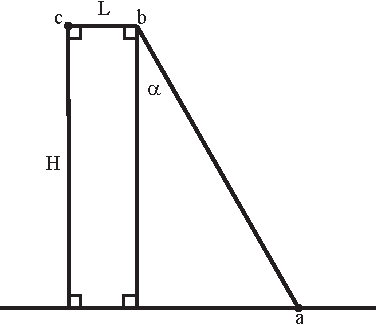
\includegraphics[width=0.5\linewidth]{2022-2/Imagenes/Taller2/p7 diag.pdf}
    \end{figure}
\end{multicols}




% Para imágenes vectoriales -> el texto tiene que estar en LaTeX
% \begin{figure}[htbp]
%   \centering
%   \svgpath{../Imagenes/ejercicios}  -> .. irse pa'trás 
%   \includesvg{ej5.svg}
% \end{figure}

\end{enumerate}
\end{document}
